\section{\infinitejest as a Network}

Our network represents characters as nodes and character co-mentions as weighted edges. The more of often two characters are mentioned in proximity to each other, the greater the weight of the edge between them. Our approach gives an extremely broad view of a book as a network of character co-mentions.

Our choice of representing characters as nodes is fairly standard, but it worth noting that there are many possible definitions of an edge in a social network: character interaction, be it verbal (in dialogue) or physical, or sentiment. 

There are certainly drawbacks to our approach -- dynamics of power between characters are entirely omitted -- but we found it still allowed us to gain insight into narrative flow and characteristics of nodes.

\subsection{Network Design}

\subsubsection{Nodes}
Network nodes constitute characters identified in the set of found named entities. These were referenced against online resources to ensure proper coverage of the characters in the book.\cite{david_foster_wallace_wiki}

\subsubsection{Edges}
Edges in the book represent a co-mention between two entities in the text. We do not match across section breaks, and we directly interpolate endnotes into the sections in which they appear. We do not interpolate endnotes referenced in an endnote into that endnote.

A threshold number of tokens (words) under which the number of tokens between the mention of one entity and another determines if an edge with weight 1 is created. If the edge already exists, the weight is incremented by 1. The current entity $i$ is only matched with proceeding entities $j$ within this threshold.

The threshold number of tokens is determined by a heuristic measure of the effect of the threshold length on the average clustering coefficient and the giant component size (see Figure \ref{fig-threshold-size}). The intuition behind these metrics is to choose the minimum threshold required to produce a giant component and a clustering coefficient that captures the highly connected nature of characters in the novel. Our threshold is 50 tokens.

\begin{figure}[ht]
    \centering
    \begin{subfigure}{0.4\textwidth}
        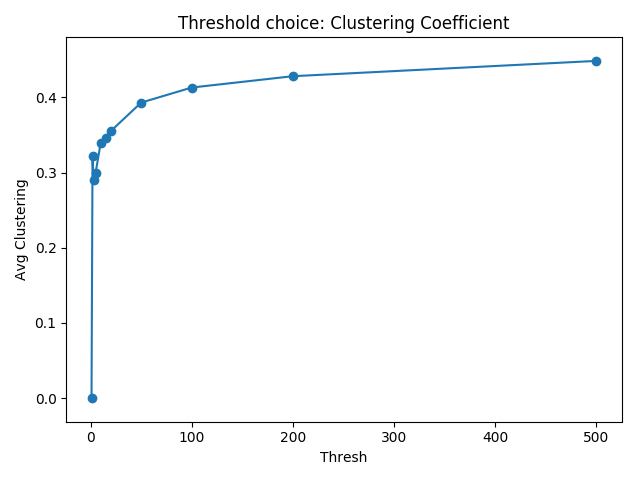
\includegraphics[width=1.\textwidth]{images/thresh_vs_avg_clustering.png}
        \caption{Edge Threshold's effect on Clustering Coefficient}
    \end{subfigure}
    \\
    \begin{subfigure}{0.4\textwidth}
        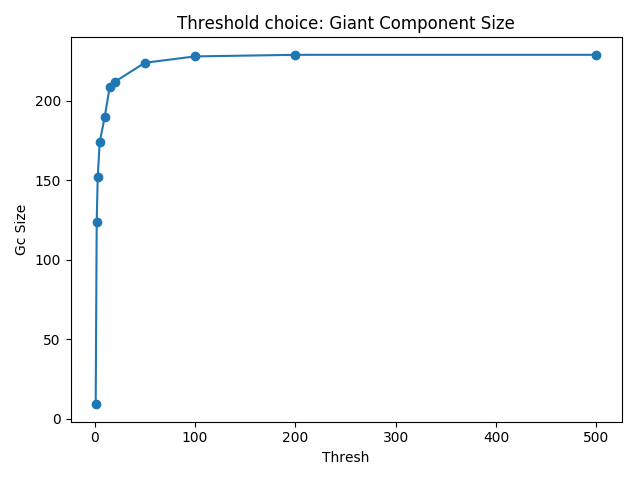
\includegraphics[width=1.\textwidth]{images/thresh_vs_gc_size.png}
        \caption{Edge Threshold's effect on the size of the Giant Component}
    \end{subfigure}
    \caption{Determining the Edge Threshold by its effect on clustering coefficient and the size of the Giant Component.}
    \label{fig-threshold-size}
\end{figure}

\subsubsection{Section as Snapshots and Modeling Recency}
In order to make comparisons between the book's ordering of events ('booktime') and the chronological ordering, we constructed a timelapse of graph snapshots that represents the aggregate graph structure up to the current section in the given ordering. Regardless of the ordering, the graph at the end of each sequence is identical. To model the differences in exposure to narratives and characters between the two orderings, we add a mechanism to decay the weights of the graph. Whenever a section is applied to the cumulative network, that section's weights are passed through a decay function orginially developed by psychologist Hermann Ebinghaus dubbed a `forgetting curve'. This curve is as follows:

\begin{equation}
    R = e^{\frac{-t}{(10000*s)}}
\end{equation}

Here $R$ represents the memory retention. $t$ represents the time (the number of tokens in the section). $s$ represents memory stability. The exponent is scaled by $\frac{1}{10000}$ to ensure reasonable memory retention values between $0$ and $1$. This approach enables us build a rough model the decaying memory of a reader to the narrative and character exposure differences between `chronological' and `booktime' section orderings.
